\documentclass[11pt]{article} %Sets the default text size to 11pt and class to article.
%------------------------Dimensions--------------------------------------------
\topmargin=0.0in %length of margin at the top of the page (1 inch added by default)
\oddsidemargin=0.0in %length of margin on sides for odd pages
\evensidemargin=0in %length of margin on sides for even pages
\textwidth=6.5in %How wide you want your text to be
\marginparwidth=0.5in
\headheight=0pt %1in margins at top and bottom (1 inch is added to this value by default)
\headsep=0pt %Increase to increase white space in between headers and the top of the page
\textheight=9.1in %How tall the text body is allowed to be on each page

\usepackage{hyperref}
\usepackage[usenames,dvipsnames]{color}
\usepackage{paralist}
\usepackage{amsmath}
\usepackage{graphicx}
\usepackage[font=small,labelfont=bf]{caption}

\begin{document}

\title{Thesis Proposal: Scalable Systems and \\ Algorithms for Genomic Variant Analysis}
\author{Frank Austin Nothaft} 
\date{}

\maketitle

\begin{abstract}

Recent improvements in DNA sequencing technologies have dropped the cost of sequencing a
human genome to under \$1,000. This drastic economic change has enabled both the use of
sequencing in clinical medicine and the genotyping of large cohorts. However, this shift
brings new problems: the cost of analyzing genomic data is growing as quickly as the cost
of collecting genomic data is falling. This trend is occurring because the decline in the
cost of sequencing is outpacing Moore's law.

Genomics is experiencing quintessential ``big data'' problems. To uncover the link between
genomic variation and traits, we need to statistically analyze large cohorts. Because each
genome represents $\mathcal{O}(1-100\text{GB})$ of data, moderately sized cohorts like the
1,000 Genomes project (which contains more than 70TB of data) present significant data
storage and processing challenges. By collecting and processing this data, we are able to
uncover statistical linkages between genomic variation and diseases. However, these statistical
correlations do not always provide biological insight: in some cancers, such as Acute
Myeloid Leukemia~(AML), very few genes are modified by mutations. In diseases like AML,
we need to make use of both statistical links and novel genomic annotation techniques to
understand the underlying disease process.

This problem requires a two pronged approach that tackles both infrastructural and
algorithmic problems. We have developed the \textsc{ADAM} system, which provides an efficient
API for distributing genomic analyses across many nodes. On top of \textsc{ADAM}, we are
building \textsc{Avocado}, a distributed variant caller that introduces efficient algorithms
for identifing genomic variants. In addition to having lower runtime complexity than prior
variant detection algorithms, the core algorithm in \textsc{Avocado} computes canonical
representations of variation, which simplifies downstream statistical analyses. To enable
very large scale genotype-phenotype association queries, we are building \textsc{Gnocchi},
a map-reduce based statistical query engine. Finally, we are developing a novel algorithm,
\textsc{Fig}, which can be used to identify variants that modify the effect of regulatory
protein binding sites in the genome. By understanding how genome variation can impact
transcriptional regulation, we hope to better understand complex diseases like AML.

\end{abstract}

\section{Thesis Statement}

Although all cancers are defined by a set of mutations that distrupt the normal function
of the genome, these mutations often occur at low frequencies. To understand the biology
behind these low frequency mutations, we need to run large scale ($\mathcal{O}(>100,000)$
individuals) statistical analyses. Although the cost of genome sequencing has plummeted
in the last fifteen years, the analysis of large cohorts is limited by the computational
cost of analysing large quantities of genomic data. To make these analyses tractible, we
must enable the use of novel parallel computing technology, and development more efficient
genome analysis algorithms. By coupling these improved analyses with advanced genomic
annotation algorithms, we can better understand the role of variants in non-coding regions
of the genome, and their impact on diseases like AML.

\section{Background}

Since the completion of the Human Genome Project in 2003, genome sequencing costs have dropped
by more than $10,000\times$~\cite{nhgri}. The rapidly declining cost of sequencing a single human
genome has enabled large sequencing projects like the 1,000 Genomes Project~\cite{siva08} and
the Cancer Genome Atlas~(TCGA,~\cite{weinstein13}). As these large sequencing projects perform
analysis that process terabytes to petabytes of genomic data, they have created a demand
for genomic analysis tools that can efficiently process these scales of
data~\cite{schadt10, stein10}. Figure~\ref{fig:sequencing-costs} juxtaposes the rapid drop
in the cost of sequencing a single genome against the amount of data collected by each successive
generation of sequencing projects. New DNA sequencers such as the Illumina X10 provide
sufficient throughput such that a single hospital or research lab can generate 750GB of genomic
data per day, or 275TB of genomic data per year~\cite{illumina-x10}.

\begin{figure}[h]
\begin{center}
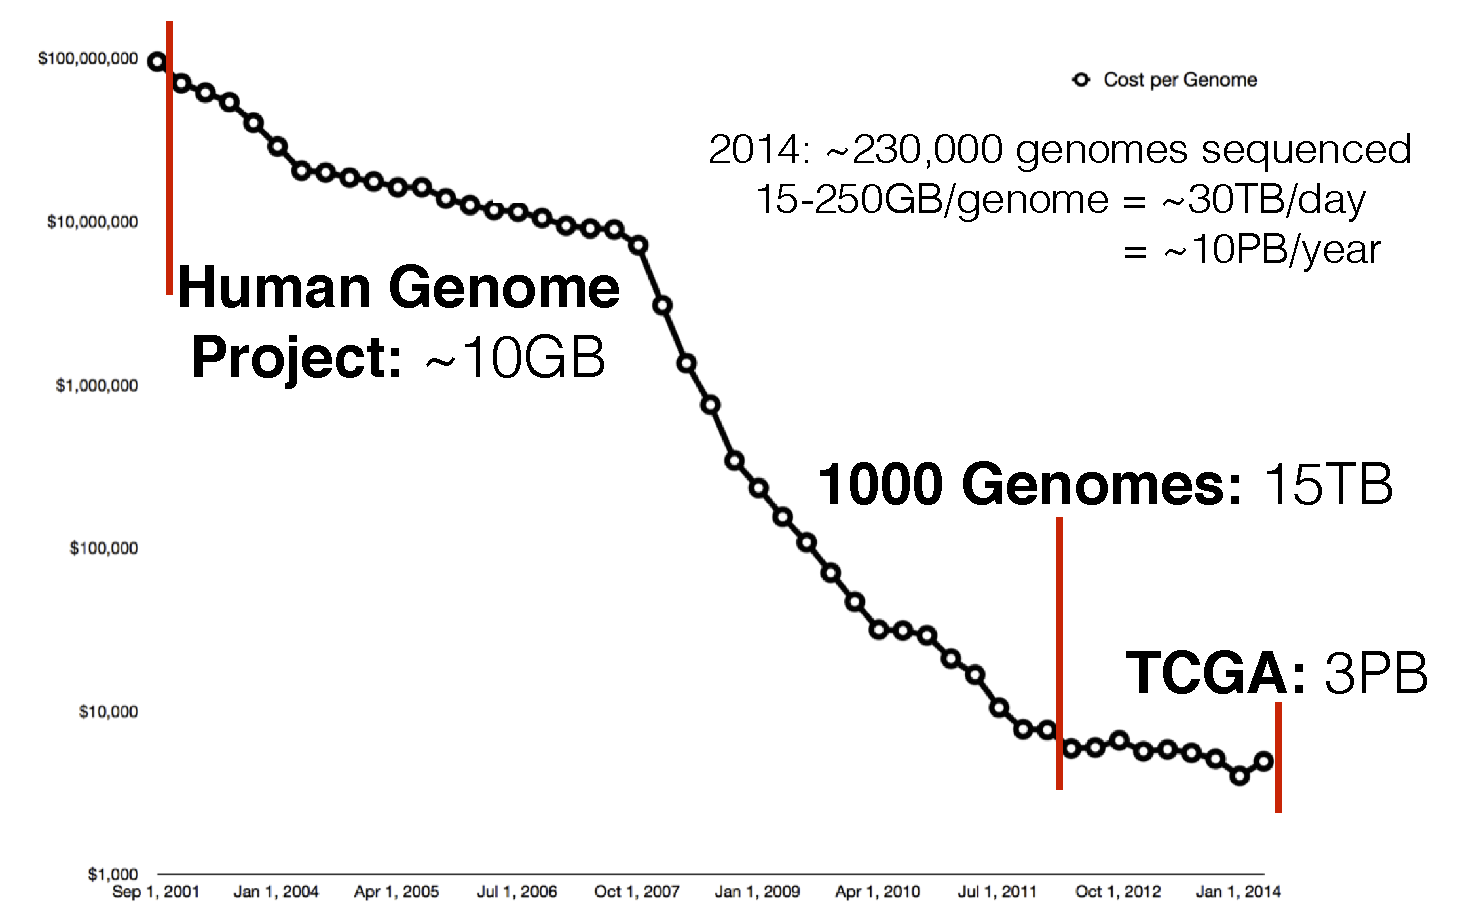
\includegraphics[width=0.6\linewidth]{genome-sequencing.pdf}
\caption{Genome sequencing costs over time, from NHGRI numbers~\cite{nhgri}, with
data volumes of major genome sequencing projects overlaid.}
\label{fig:sequencing-costs}
\end{center}
\end{figure}

Over a similar time range, commercial needs led to the development of horizontally scalable
analytics systems. The development and deployment of \textsc{MapReduce} at
Google~\cite{dean04, dean08} spawned the development of a variety of distributed analytics tools
and the \textsc{Hadoop} ecosystem~\cite{hadoop}. In turn, these systems led to other systems
that provided a more fluent programming model~\cite{yu08} and higher performance~\cite{zaharia10}.
The demand for these systems has been driven by the increase in the amount of data available to
analysts, and has coincided with the development of statistical systems that are accessible to
non-experts, such as \textsc{Scikit-learn}~\cite{pedregosa11} and \textsc{MLI}~\cite{sparks13}.

With the rapid drop in the cost of sequencing a genome, and the accompanying growth in available data,
there is a good opportunity to apply modern, horizontally scalable analytics systems to genomics. New
projects such as the 100K for UK, which aims to sequence the genomes of 100,000 individuals in the
United Kingdom~\cite{uk100k}, and the Department of Veterans Affairs' Million Veteran project~\cite{mvp}
will generate three to four \emph{orders of magnitude} more data than prior projects like the 1,000
Genomes Project~\cite{siva08}. Additionally, periodic releases of new reference datasets such as reference
genomes necessitates the periodic re-analysis of these large datasets. These projects use the current ``best
practice'' genomic variant calling pipelines~\cite{auwera13}, which takes approximately 120 hours to
process a single, high-quality human genome using a single, beefy node~\cite{talwalkar14}. To address
these challenges, scientists have started to apply computer systems techniques such as
map-reduce~\cite{langmead09, mckenna10, schatz09} and columnar storage~\cite{fritz11} to custom
scientific compute/storage systems. While these systems have improved analysis cost and performance,
current implementations incur significant overheads imposed by the legacy formats and codebases that
they use.

Additionally, although these experiments have provided us with a large set of data about
human variation, several large questions remain. One large question pertains to the role of
variation that occurs outside of the coding portions of the human genome. Although the human
genome is more than three billion bases long, the portion of the genome that codes for proteins
(the exome) is only approximately 1\% of the genome. Although we can predict how modifications
to DNA sequence inside of the exome will modify the structure and composition of
proteins~\cite{mclaren10}, no such rules exist for the remaining 99\% of the genome. However,
81\% of the sequence outside of the exome is responsible for regulating the rate at which
a gene in the exome is translated into a protein~\cite{gerstein12}. This estimate was derived
by identifying the positions where transcription factors~(TFs\footnote{Transcription factors are
proteins whose function is to bind to DNA and control the rate at which DNA is transcribed into
RNA. This RNA can then be translated into a protein.}) attach to the genome. As we show in
Figure~\ref{fig:tfbs}, sequence variants that occur in regulatory regions can modify the rate
at which nearby genes are transcribed and translated into proteins~\cite{levo14, weingarten14}.

\begin{figure}[h]
\begin{center}
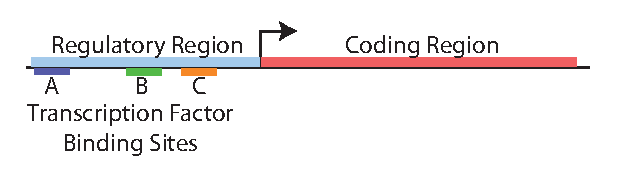
\includegraphics[width=0.75\linewidth]{tfbs.pdf}
\caption{This figure represents the area around the start of a gene in the genome. The
arrow in the figure is the transcription start site~(TSS), which is the start of the coding
portion of the gene. In the 1,500 bases before the TSS, there is a regulatory region where
transcription factors will bind to the genome. Variants that occur in the regulatory region
can have a variety of effects~\cite{levo14, weingarten14}. For example, a variant that occurs
at TFBS A may reduce the likelihood that the TF binds. In some cases, for a TF to cause
transcription to start, it must be part of a ``complex'' of multiple TFs. If TFBS B and C
form a large protein complex, a variant that changes the distance between the two TFs (by
inserting or deleting sequence) may mean that the TFs cannot form the larger complex, and
may disable the translation of the DNA into RNA.}
\label{fig:tfbs}
\end{center}
\end{figure}

We are interested in understanding these variants so that we can understand diseases that are
known to have genomic drivers, but where few variants occur in coding sections of the genome.
One such disease is AML, which has eight clinically distinct subtypes. Although several of the
subtypes of AML are known to be caused by specific genomic variants, we do not know the drivers
for the remaining subtypes of the disease. Our understanding of variation in AML is complicated
by the relatively low rate of mutation seen in AML, versus other cancers. Figure~\ref{fig:aml}
shows the long tailed distribution of mutations in AML.

\begin{figure}[h]
\begin{center}
\includegraphics[width=\linewidth]{aml.pdf}
\caption{The nodes in this decision tree are genes known to be mutated in a patient in the LAML
subset of the TCGA~\cite{cancer13}. Each node is a gene. At each node, the left arrow indicates
that the gene was \emph{not} mutated, while the right arrow indicates that the gene was mutated.
This tree is notable because it demonstrates the long tail of mutations in AML; specifically,
the nodes running down the left side of the tree depict a large subset of patients who have
few or no coding mutations. This figure was generated by Ravi Pandya from MSR as part of the UC
Berkeley/OHSU/MSR collaboration on the BeatAML project~\cite{paten15}.}
\label{fig:aml}
\end{center}
\end{figure}

While we can use the aforementioned statistical techniques to identify correlative links
between these variants and the diseases we would like to study, these statistical techniques
do not explain the underlying disease biology, and cannot be used to determine causation.
To develop a causitive model, we build upon projects such as ENCODE~\cite{gerstein12} that
have profiled the interaction of regulatory elements with genomic sequence, While there is
an emerging literature that is studying the ``grammatical architecture'' of regulatory
regions~\cite{levo14, weingarten14}, this literature largely depends on synthetic
experiments~\cite{sharon12} to drive inference. While the results from these synthetic
experiments are valuable, and will improve our ability to model the impact of variants
on regulation, we instead seek to ask if there is a way for us to understand this relationship
from existing variation datasets? We believe we can answer these questions by building a variant
annotation engine that incorporates knowledge of this regulatory grammar, and integrating
these annotations into our correlative genomic models.

\section{Work To Date}

To address the immediate computational needs of sequencing analyses, we embarked on the design of
the \textsc{ADAM} system~\cite{massie13, nothaft15}. \textsc{ADAM} is a genomic processing system
that was built using open source technologies that are designed for data intensive computing, such
as Apache \textsc{Parquet}~\cite{parquet} and \textsc{Spark}~\cite{zaharia12, zaharia10}. The main
goal of building the \textsc{ADAM} system was to demonstrate that a well architected system that
was built using commodity technologies could outperform optimized, genomics-specific systems,
while letting bioinformaticians write genomic analyses using higher level primitives.

To make it possible to program genomic analyses against higher level abstractions, we created the
decomposed stack shown in Figure~\ref{fig:stack-model}, which was inspired by the stack models
common in networking~\cite{zimmermann80}. The key feature of this stack model is the use of a
schema to describe the data we are processing. Conventional genomics pipelines rely on binary
data formats that do not distinguish the logical structure of data from the physical representation
of data. This is problematic, as legacy genomic formats such as SAM/BAM~\cite{li09} use the
blurring of lines between logical and physical representations to perform ``optimizations''
that make analyses brittle to write. In the popular \textsc{Genome Analysis Toolkit}~(GATK,
\cite{mckenna10}), analyses are written against the ``walker'' API, which presents a sorted
iterator over the genome. By blurring the bounds between the logical and physical views of the
data, the \textsc{GATK} can accelerate ``walker'' traversals by pushing a sort order invariant
down into the data. However, as we have shown in prior work~\cite{nothaft15}, this approach
can lead to subtle algorithm correctness bugs. In this prior work, we demonstrate how these
same algorithms can be written using common relational primitives such as aggregates and joins,
and we show that this allows us to scale genomic analyses linearly to run on thousands of cores.

\begin{figure}[h]
\begin{center}
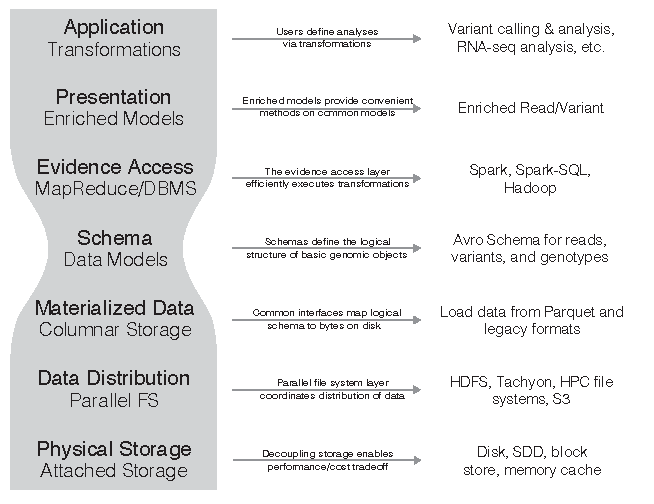
\includegraphics[width=0.6\linewidth]{../ms-thesis/expanded-stack-2.pdf}
\caption{A Stack Model for Genomic Analyses}
\label{fig:stack-model}
\end{center}
\end{figure}

As a continuation of this work, we are working on a manuscript that demonstrates how \textsc{ADAM}
can be used to improve the performance of conventional variant calling pipelines, without
sacrificing accuracy. To do this, we have evaluated a hybrid variant calling pipeline that uses
\textsc{ADAM}, along with the \textsc{GATK}'s \textsc{HaplotypeCaller}~\cite{depristo11}. We
have compared this to the \textsc{GATK}'s ``Best Practices'' pipeline~\cite{auwera13}, and have
been able to achieve a $3\times$ latency improvement while improving cost by $2\times$. The
two pipelines generate statistically equivalent variant calls. As part of the manuscript, we
will demonstrate how \textsc{ADAM} makes it less expensive to process large genomic datasets
by recalling the 50TB Simons Genome Diversity Dataset~\cite{simons}.

We have been developing several tools that run on top of the \textsc{ADAM} processing framework.
One of these tools is the \textsc{Avocado} variant caller, which we aim to use to replace the
\textsc{GATK}. \textsc{Avocado} is a fully distributed variant caller, which calls variants using
a local reassembly strategy. We are in the process of preparing a manuscript on the novel local
reassembly algorithm used by \textsc{Avocado}. While realignment and reassembly based algorithms
are used in all common variant callers~(such as the \textsc{GATK}'s \textsc{HaplotypeCaller},
\textsc{Platypus}~\cite{rimmer14}, and \textsc{Scalpel}~\cite{narzisi14}), these algorithms are
slow due to their high runtime complexity. These algorithms use a graph-theoretic algorithm to
assemble potential haplotypes from the reads around a putative variant locus. However, these
algorithms achieve poor throughput because of the existance of a $\mathcal{O}(n^2)$ stage
where all haplotype-read pairs are scored. In \textsc{Avocado}, we exploit the structure of the
\emph{de Bruijn} graph that is assembled from the reads at the locus to achieve $\mathcal{O}(n)$
performance. Additionally, our algorithm provides provably canonical representations of insertion
and deletion variants, which simplifies the joint analysis of multiple samples.

\section{Proposed Work}

I plan to tackle three remaining problems:

\begin{itemize}
\item How can we use the efficient algorithms in \textsc{ADAM} and \textsc{Avocado} to jointly
analyze thousands of samples?
\item How can we parallelize the statistical analysis of genotype-phenotype associations on
large cohorts?
\item Can we use genomic annotations to better understand the impact of low frequency variation
on transcriptional regulation?
\end{itemize}

As mentioned earlier, we have already demonstrated the potential of \textsc{ADAM} for acheving
order-of-magnitude improvements in throughput when processing a single sample, and we have
shown how we can use the efficient algorithms in \textsc{Avocado} to achieve faster region
reassembly. Currently, memory capacity backpressure limits the number of genomes we can process
given a fixed amount of hardware. This is caused by metadata that is replicated when we translate
data between \textsc{Parquet}'s columnar format on disk and \textsc{Spark}'s row oriented format
in memory. However, we have recently experimented with a hybrid denormalized columnar scheme and
have reduced our memory consumption by $11\times$.

Along with this, we are working on several other parallel data translation problems. Specifically,
while we introduced optimized join algorithms for finding overlapping genomic regions in the
latest \textsc{ADAM} paper~\cite{nothaft15}, we are working on a further optimizations to these
join algorithms for joint variant calling. When jointly analyzing multiple genomes, we perform a
sweeping pass over the genome in coordinate space. Although this approach is implicitly serial,
we are working to express this algorithm as an adaptive self join. The adaptive portion of this
join selects the granularity used for computing key equality. In areas of the genome where there
are no insertion or deletion variants, we work at single base pair granularity. This granularity
expands to match the size of the largest deletion whenever one is present. By using this self join
instead of a na\"{i}ve algorithm that divides the genome into fixed size chunks, we will be able
to increase our parallelism while reducing the instantaneous amount of data that we materialize
into memory and preserving the ability to call deletion variants.

Although tools such as \textsc{PLINK}~\cite{purcell07, chang15} can already be used to run
genotype-phenotype analyses, these tools have largely been designed to work with legacy genetic
data. The data generated by modest sized sequencing experiments (such as the 1,000 Genomes project,
which has 1.8TB of genotypic data) has grown to the point where the data is too large to fit in
memory on a single machine. To work around this, these tools rely on ad hoc parallelization
methods~\cite{chang15}, such as parallel script dispatch. These ad hoc methods are both
inefficient and prone to machine failures, and cannot make use of efficient distributed file
systems, like \textsc{HDFS}. The I/O patterns of genotype-phenotype analyses that are run on
genotypes generated by next generation sequencing workflows are particularly inefficient, as
these queries only touch select fields from the genotype data, but must read the entirety of each
VCF genotype record. By building \textsc{Gnocchi}, a genotype-phenotype correlation engine, on top
of \textsc{ADAM}, we will be able to make use of our columnar file format to eliminate the I/O
bottleneck present in current genotype-phenotype tools and to enable the efficient parallelization
of genotype-phenotype analyses to hundreds of machines. To date, we have implemented a case-control
model for use in parallel genome wide association studies~(GWAS), which we are in the process of
validating. We plan to extend \textsc{Gnocchi} to support a more general set of statistical models.

Additionally, with the work on genotype clustering in \textsc{Gnocchi}, we see a great
opportunity to make a contribution to the state-of-the-art in scalable systems for machine
learning. While recent research at the intersection of computer systems and machine learning
has focused on algorithms for training a single statistical model on systems that are ``tall
and skinny''~\cite{meng15, zadeh15}, genomics exhibits neither of these characteristics.
Unlike Internet scale companies, where feature vectors are small and there are many users,
feature vectors for genomic datasets are comprised of all of the genotypes seen for an
individual sample. For a whole genome sequencing run, this sparse vector can represent more
than 1 million genotypes. Although fast algorithms are known for fitting linear mixed
models~\cite{lippert11} for learning genotype-phenotype correlations, there has not been
significant research into fast clustering methods for ``wide and flat'' data. In preliminary
work, we have found that sampling-based approaches can be used to efficiently apply parallel
methods for clustering on tall and skinny datasets~\cite{bahmani12, meng15} to this wide and
flat data, but at the loss of some accuracy. We will improve our clustering accuracy by deriving
efficient parallel methods that are optimized for wide and flat data.

While genotype-phenotype analyses can generate correlative findings, these findings do not
necessarily shed light on the underlying biology that drives these correlations. This is
particularly troublesome for the non-coding regions of the genome, where traditional variant
effect annotation methods that look for impacts on protein composition cannot be
used~\cite{mclaren10}. We have done some preliminary investigations to see how variation impacts
the regulatory regions upstream of the transcription start site~(TSS) of a gene. We implemeneted
this as part of the \textsc{Fig} tool, which is an \textsc{ADAM}-based engine for annotating
genomic variants. In this preliminary experiment, we searched for variants from phase 3 of the
1,000 Genomes project that modified transcription factor binding affinity or spacing. Since
Transcription Factor Binding Site~(TFBS) spacing requires knowledge about whether two TFBS are
on the same strand of DNA, we made use of the phasing from the 1,000 Genomes project to annotate
phased haplotypes. To annotate TFBSs, we used data from the ENCODE project that was compiled by
Kheradpour and Manolis~\cite{kheradpour14} and the GRCh37 gene annotations.

Our preliminary experiments showed several interesting results. First, we found that the regulatory
regions upstream of the TSS have a lower rate of variation than expected. 43\% of the annotated
regions did not contain variants, which is lower than expected as the rate of common variation
in the human genome is 0.1\%\footnote{This rate underestimates the rate of variation in a single
individual. This estimate is derived from the 1,000 Genomes project, where one ``common'' variant
(present in $>5\%$ of the population) were seen per 1,000bp.}. Under a Binomial distribution with
$p = 0.001$ and $n = 1500$, we expect only 22\% of regions to not have variants. This implies that
these regions are evolutionarily conserved. However, we did see several regions where more than
three TFBSs were lost, which warrants further investigation. Additionally, we found that these
variants were unlikely to modify the binding affinity of TFBSs. Binding compatibility was lost at
fewer than 1\% of sites, and binding affinity was decreased at approximately 10\% of sites.

Ultimately, we would like to unify the annotations generated by \textsc{Fig} with the associations
generated by \textsc{Gnocchi}. By applying these methods to a large dataset, such as the
GEUVADIS subset of the 1,000 Genomes project~\cite{lappalainen13}, we will be able to verify
whether the synthetic models for regulatory grammar~\cite{levo14, sharon12, weingarten14}
are applicable in vivo. Additionally, this work will serve as a valuable way to calibrate the
functional annotations generated by \textsc{Fig}. Although we have gained TFBS data from the
ENCODE project~\cite{gerstein12, kheradpour14}, it is unlikely to believe that all predicted
TFBS have an equal impact on transcriptional regulation across all genes. By feeding this data
back into the \textsc{Fig} annotation engine, we can better predict the effect of variants
that occur in the regulatory regions. With this knowledge, we can better understand the role
of the non-coding variants in diseases by being able to predict the impact of these variants
on gene expression.

\bibliographystyle{acm}
\bibliography{thesis-proposal}

\end{document}
